% AIIT Bulletin Template Version 18.0 2024-07-09

\documentclass[a4paper, 9pt, twocolumn]{extarticle}
\usepackage{variables}
\title{AIIT bulletin format: English version \YEAR}
\author[1*]{Minoru Matsui}
\author[1,2]{Kyodo Shippitsusha}
\author[2,3]{Saishu Shippitsusha}
\affil[1]{Advanced Institute of Industrial Technology}
\affil[2]{Tokyo Metropolitan University}
\affil[3]{Tokyo Metropolitan College of Industrial Technology}
\affil[*]{Corresponding author: Minoru Matsui, xerroxcopy@gmail.com}
\newcommand{\abstractcontent}{Write in English. Lorem ipsum dolor sit amet, consectetur adipiscing elit. Suspendisse ac enim turpis. Morbi eu maximus velit, ac maximus enim. Phasellus et pellentesque ante. Pellentesque non velit id tortor rutrum pretium a ac neque. Sed congue sit amet leo vel laoreet. Vivamus ullamcorper a dolor in aliquet. Pellentesque finibus at nunc ac egestas. Proin eu sollicitudin nisi. Sed cursus pulvinar leo. In erat erat, molestie ac euismod at, egestas non neque. Nam viverra nunc erat, vitae elementum tortor cursus et. Duis sed magna vel turpis congue finibus.Morbi pulvinar auctor quam eget commodo. Quisque mi nulla, tempor quis sem sed, auctor pharetra turpis. Cras blandit vestibulum dapibus. Sed ac nisi et metus sollicitudin tincidunt rutrum eget felis. Donec imperdiet dolor nec elit interdum, vitae ultrices turpis consectetur. Sed lacinia tempus lacinia. Morbi facilisis metus ac diam sollicitudin, et ornare urna rutrum. Nullam sollicitudin fringilla ipsum, nec vulputate risus. Sed sit amet euismod nulla.Proin porttitor diam ac lacus vehicula facilisis. Sed at tempus magna. Aenean eget vehicula ipsum, non porta arcu. Suspendisse vitae lacinia leo. Ut sit amet purus imperdiet ipsum tempor efficitur auctor eget magna. Phasellus suscipit risus eu semper eleifend. Ut tempor magna viverra urna condimentum, sed pretium ipsum iaculis. Pellentesque aliquet tincidunt felis ac imperdiet.Phasellus viverra tristique lorem, in dignissim risus bibendum non. Praesent varius urna eget nibh lacinia, sed faucibus turpis tristique. Proin hendrerit pretium ullamcorper . Donec non vestibulum diam. Sed suscipit, justo sit amet auctor aliquam, orci sem sollicitudin lacus, et maximus. (max 250 words)}
\newcommand{\keywordscontent}{keyword1; keyword2; keyword3 (max 5 keywords)}
% import a package set
\usepackage{aiit}

% load settings for layouts and aesthetic tweaks. 
% comment this out to speed up compile (draft quality)
\usepackage{aiit-aes-en}

\begin{document}
% AIIT Bulletin Template Version 17.9 2023-07-13; Equivalent Word template version: 5

% the vspace is slightly different from Japanese version.
\pagestyle{aiit}
\twocolumn[%
\vspace{-11mm}
\maketitle
\vspace{-13mm}
\begin{onecolabstract}
\abstractcontent
\end{onecolabstract}
\small\textbf{Keywords\quad}\keywordscontent\\
\vspace{2mm}
\rule{\textwidth}{.1mm}
\vspace{8mm}
]



\section{Introduction}

Write in English. Lorem ipsum dolor sit amet, consectetur adipiscing elit. Suspendisse ac enim turpis. Morbi eu maximus velit, ac maximus enim. Phasellus et pellentesque ante. Pellentesque non velit.

Nam viverra nunc erat, vitae elementum tortor cursus et. Duis sed magna vel turpis congue finibus.Morbi pulvinar auctor quam eget commodo. Quisque mi nulla, tempor quis sem sed, auctor pharetra turpis. Cras blandit vestibulum dapibus. Sed ac nisi et metus sollicitudin tincidunt rutrum eget felis. Donec imperdiet dolor nec elit interdum, 

\subsection*{Literature review}

Nullam sollicitudin fringilla ipsum, nec vulputate risus. Sed sit amet euismod nulla.Proin porttitor diam ac lacus vehicula facilisis. Sed at tempus magna. Aenean eget vehicula ipsum, non porta arcu. Suspendisse vitae lacinia leo. Ut sit amet purus imperdiet ipsum tempor efficitur auctor eget magna. Phasellus suscipit risus eu semper eleifend. Ut tempor magna viverra urna condimentum, sed pretium ipsum iaculis. Pellentesque aliquet tincidunt felis ac imperdiet.Phasellus viverra tristique lorem, in dignissim risus bibendum non. 

Praesent varius urna eget nibh lacinia, sed faucibus turpis tristique. Proin hendrerit pretium ullamcorper . Donec non vestibulum diam. Sed suscipit, justo sit amet auctor aliquam, orci sem sollicitudin lacus, et maximus\cite{Cooney2017-yt}.

Fig. \ref{figure:figureExample}, Table \ref{table:tableExample}, \verb|date|, \mintinline{r}{function(x) {x + 1}}, Equation \eqref{eq:example}
\begin{figure}[hbt!]
  \centering
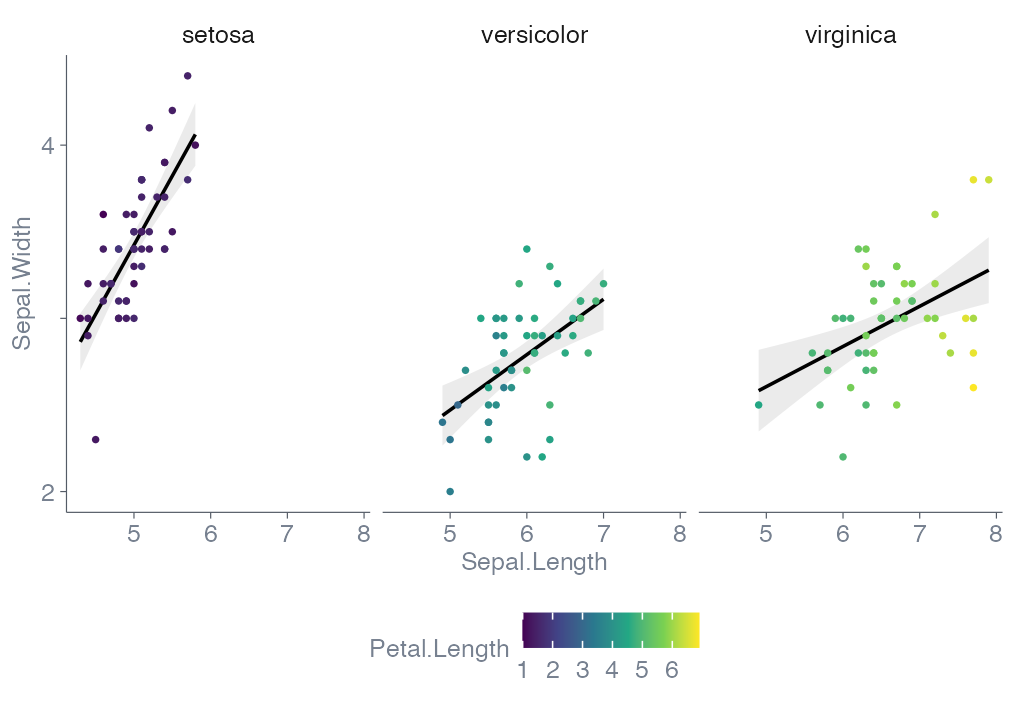
\includegraphics[width=89mm]{p_plot}
    \caption{89 mm}
    \label{figure:figureExample}
\end{figure}
\begin{figure*}[hbt!]
  \centering
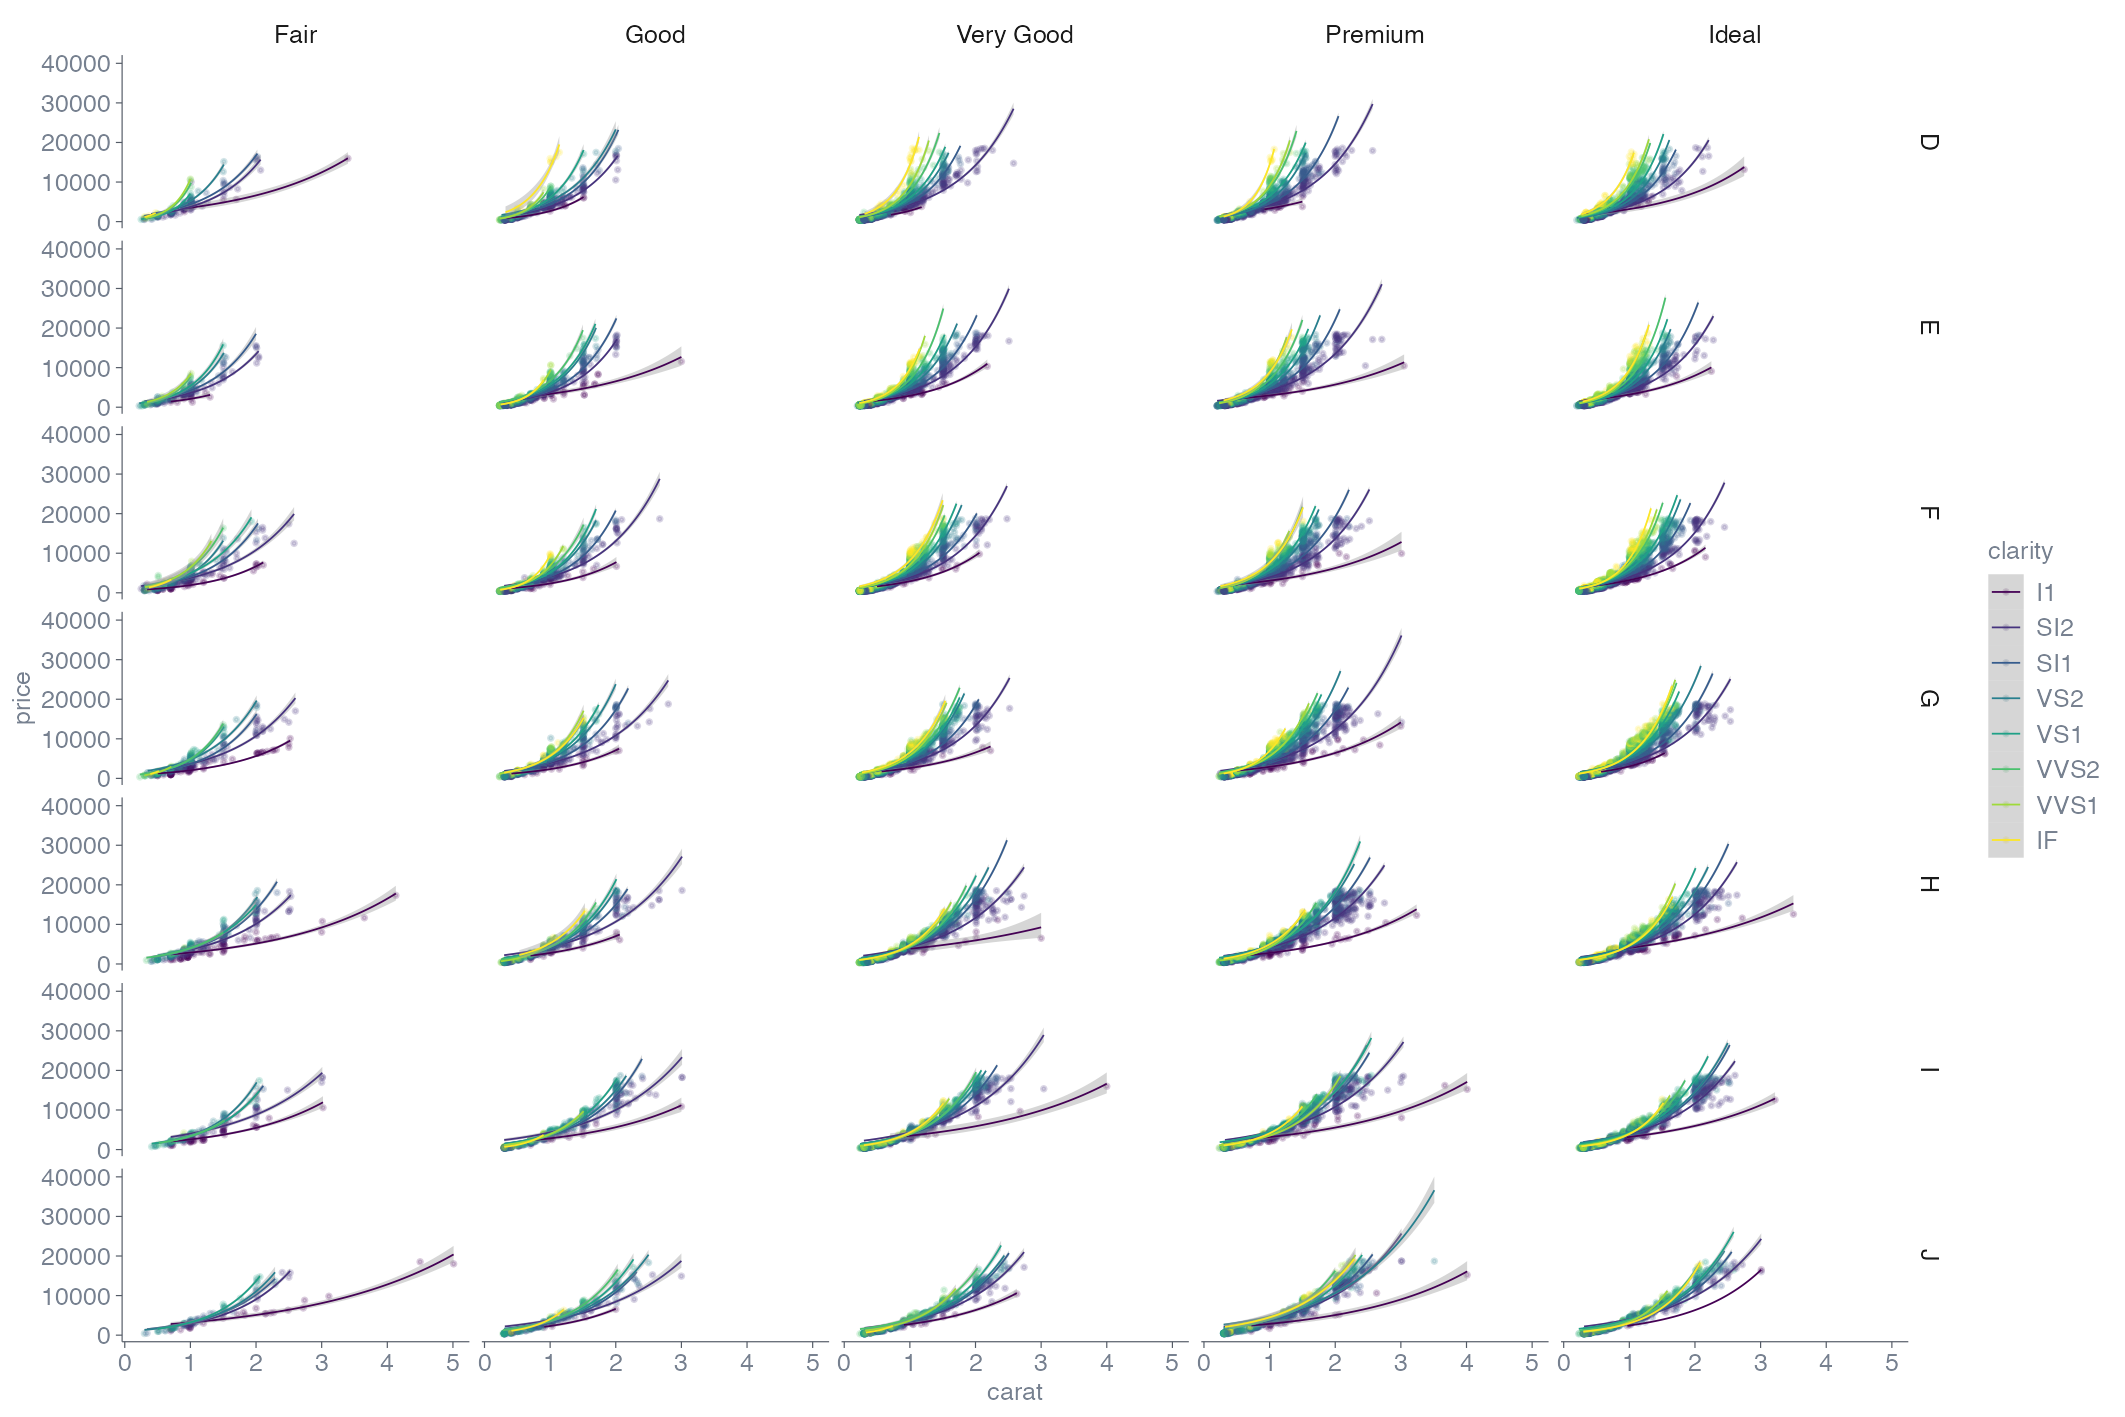
\includegraphics[width=\textwidth]{p_plot2}
    \caption{186 mm}
    \label{figure:figureExampleLarge}
\end{figure*}



\begin{table}[hbt!]
 \caption{An example of a table}
 \label{table:tableExample}
 \centering
    \begin{tabular}{lllll}
        \toprule
        \multirow{2}{*}{Models} & \multicolumn{3}{c}{Metric 1} & Metric 2\\
        \cmidrule{2-4} \cmidrule{5-5} \\
        {} & precision & recall & F-score  & R@10 \\
        \midrule
        model 1 & 0.67  & 0.8 & 0.729  & 0.75 \\
        model 2 & 0.8 & 0.9 & 0.847 & 0.85 \\
        \bottomrule
    \end{tabular}
\end{table}



\begin{minted}{r}
library(tidyverse)
theme_aiit <- 
  theme_minimal(6, base_family = "Helvetica") +
  theme(
    line = element_line(linewidth = .1/.75, colour = "#545B66"),
    text = element_text(size = 6, colour = "#778190"),
    title = element_text(size = 6, colour = "#778190"),
    panel.grid = element_blank(),
    axis.line = element_line(),
    axis.text = element_text(size = 6, colour = "#778190"),
    axis.ticks = element_line(),
    plot.background = element_rect(fill = "white", colour = NA),
    strip.text = element_text(size = 6),
    strip.switch.pad.grid = unit(2, "mm"),
    strip.placement = "outside",
    legend.text = element_text(size = 6),
    legend.key.size = unit(3, units = "mm"),
    plot.tag = element_text(
      size = 10, 
      family = "Helvetica", 
      face = "bold"
    )
  )
\end{minted}
For Fig. \ref{figure:figureExample},

\begin{minted}{r}
iris |> 
  ggplot(
    aes(
      x = Sepal.Length, 
      y = Sepal.Width, 
      colour = Petal.Length, 
      group = Species)
  ) +
  geom_smooth(
    method = "lm", 
    size = .3/.75, 
    colour = "black", 
    fill = "grey80"
  ) +
  geom_point(size = .15/.75) +
  scale_x_continuous(breaks = 5:8) +
  scale_y_continuous(breaks = 2:4, labels = c(2, "", 4)) +
  scale_colour_viridis_c() +
  facet_wrap(vars(Species)) +
  theme_aiit +
  theme(legend.position = "bottom")
ggsave("./output/p_plot.png", width = 86, height = 60, unit ="mm", dpi = 600)
\end{minted}

For Fig. \ref{figure:figureExampleLarge},

\begin{minted}{r}
diamonds |> 
  ggplot(aes(carat, price, colour  = clarity)) +
  geom_point(size = .15/.75, alpha = .2) +
  geom_smooth(
    method = "glm", 
    method.args = list(family = gaussian(link = "log")),
    size = .2
  ) +
  facet_grid(cols = vars(cut), rows = vars(color)) +
  scale_colour_viridis_d() +
  theme_aiit
ggsave("./output/p_plot2.png", width = 180, height = 120, unit = "mm", dpi = 600)
\end{minted}



\begin{equation}
\left( \int_0^\infty \frac{\sin x}{\sqrt{x}} dx \right)^2=
\sum_{k=0}^\infty \frac{(2k)!}{2^{2k}(k!)^2} \frac{1}{2k+1}=
\prod_{k=1}^\infty \frac{4k^2}{4k^2 -1}= \frac{\pi}{2} \label{eq:example}
\end{equation}

\begin{equation}
  c = 299{,}792{,}458 \, \mathrm{m/s}
\end{equation}

\begin{equation}
  A = \begin{pmatrix}
        a_{11} & \ldots & a_{1n} \\
        \vdots & \ddots & \vdots \\
        a_{m1} & \ldots & a_{mn}
      \end{pmatrix}
\end{equation}

\printbibliography
% select an applicable license from the list below and comment out (or delete) the others
\vspace{8mm}
\noindent

\includegraphics[height=8mm]{licenses/by}
\vspace{2mm}
\begin{spacing}{.6}
\noindent
\textbf{Open Access} This article is licensed under CC BY 4.0. To view a copy of this license, visit \url{https://creativecommons.org/licenses/by/4.0/}
\end{spacing} 
% \vspace{8mm}
\noindent

\includegraphics[height=8mm]{licenses/by-sa}

\begin{spacing}{.6}
\noindent
\textbf{Open Access} This article is licensed under CC BY-SA 4.0. To view a copy of this license, visit \url{https://creativecommons.org/licenses/by-sa/4.0/}
\end{spacing} 
% \vspace{8mm}
\noindent

\includegraphics[height=8mm]{licenses/by-nd}

\begin{spacing}{.6}
\noindent
\textbf{Open Access} This article is licensed under CC BY-ND 4.0. To view a copy of this license, visit \url{https://creativecommons.org/licenses/by-nd/4.0/}
\end{spacing} 
% \vspace{8mm}
\noindent

\includegraphics[height=8mm]{licenses/by-nc}

\begin{spacing}{.6}
\noindent
\textbf{Open Access} This article is licensed under CC BY-NC 4.0. To view a copy of this license, visit \url{https://creativecommons.org/licenses/by-nc/4.0/}
\end{spacing} 
% \vspace{8mm}
\noindent

\includegraphics[height=8mm]{licenses/by-nc-sa}

\begin{spacing}{.6}
\noindent
\textbf{Open Access} This article is licensed under CC BY-NC-SA 4.0. To view a copy of this license, visit \url{https://creativecommons.org/licenses/by-nc-sa/4.0/}
\end{spacing} 
% \vspace{8mm}
\noindent

\includegraphics[height=8mm]{licenses/by-nc-nd}
\vspace{2mm}
\begin{spacing}{.6}
\noindent
\textbf{Open Access} This article is licensed under CC BY-NC-ND 4.0. To view a copy of this license, visit \url{https://creativecommons.org/licenses/by-nc-nd/4.0/}
\end{spacing} 
\end{document}